% Source: graduate-coursework/Prior_Semesters/Fa25/EMCH501/HW2/HW2.tex

\documentclass[border=4pt]{standalone}
\usepackage{amsmath}
\usepackage{amssymb}
\usepackage{graphicx}
\usepackage{tikz}
\usepackage{xcolor}
\usetikzlibrary{shapes.geometric, arrows.meta, positioning, decorations.pathmorphing, patterns}

\begin{document}
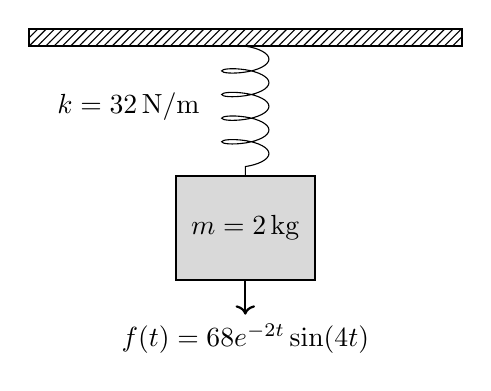
\begin{tikzpicture}[scale=1.1]
  % ceiling
  \draw[thick,pattern=north east lines] (-2.5,0) rectangle (2.5,0.2);
  \draw[thick] (-2.5,0) -- (2.5,0);
  % spring
  \draw[decoration={coil,aspect=0.3,segment length=3mm,amplitude=3mm},decorate] (0,0) -- (0,-1.5);
  \node at (-1.35,-0.7) {$k=32\,\mathrm{N/m}$};
  % mass
  \draw[fill=gray!30,thick] (-0.8,-1.5) rectangle (0.8,-2.7);
  \node at (0,-2.1) {$m=2\,\mathrm{kg}$};
  % forcing label and arrow
  \draw[->,thick] (0,-2.7) -- (0,-3.1);
  \node[below] at (0,-3.1) {$f(t)=68e^{-2t}\sin(4t)$};
\end{tikzpicture}
\end{document}
